\chapter{操作系统}

\section{操作系统}

\subsection{操作系统(Operating System)}

现代的计算机离不开操作系统(OS),操作系统是最基本也是最为重要的基础性系统软件。 \\

\begin{figure}[H]
	\centering
	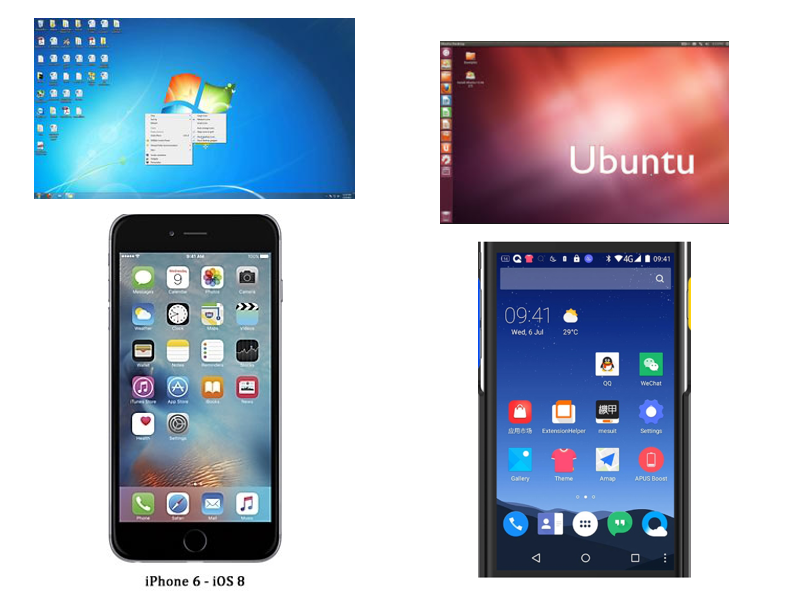
\includegraphics[scale=0.7]{img/C1/1-1/1.png}
	\caption{不同计算机的操作系统}
\end{figure}

在计算机结构中,最底层的是计算机硬件,硬件之上就是操作系统。操作系统是运行在硬件上的第一层软件,它扩展了硬件的功能。但是光有操作系统是不满足的还需要增加新的一些工具,例如开发工具和开发平台等,所以操作系统需要支持用户的程序开发。 \\

计算机结构中用户主要分为三大类:

\begin{itemize}
	\item 面向硬件的用户被称为操作系统设计者,需要熟知硬件的运行机制,以及如何在上面进行系统开发。

	\item 在操作系统纸上进行程序设计的用户被称为程序员,程序员有两种类型,一种是基于操作系统的程序设计,另一种是基于开发平台的程序设计。

	\item 终端用户(end user)直接使用应用程序。
\end{itemize}

\begin{figure}[H]
	\centering
	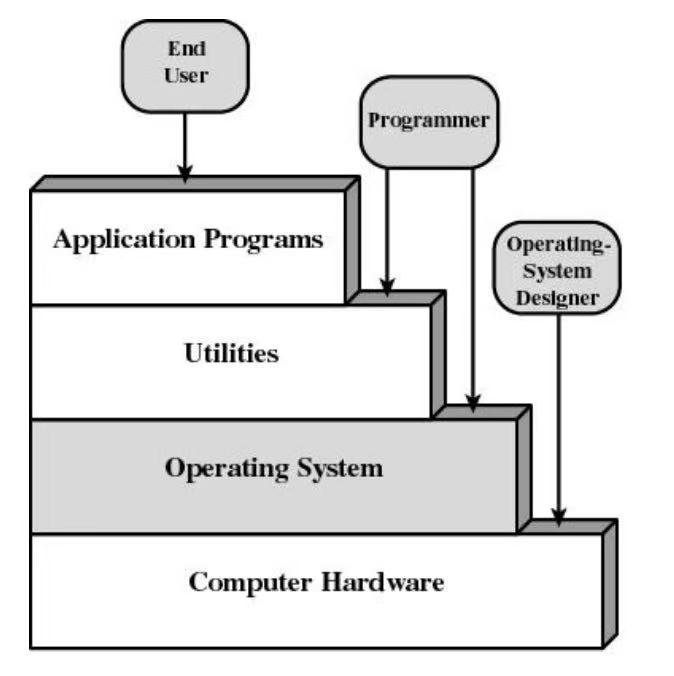
\includegraphics[scale=0.8]{img/C1/1-1/2.png}
	\caption{计算机用户层级}
\end{figure}

\subsection{操作系统观点}

现代操作系统主要有四种基本观点:

\begin{enumerate}
	\item 普通用户:OS是计算机用户使用计算机系统的接口,它为计算机用户提供而方便的工作环境。
	      \begin{figure}[H]
		      \centering
		      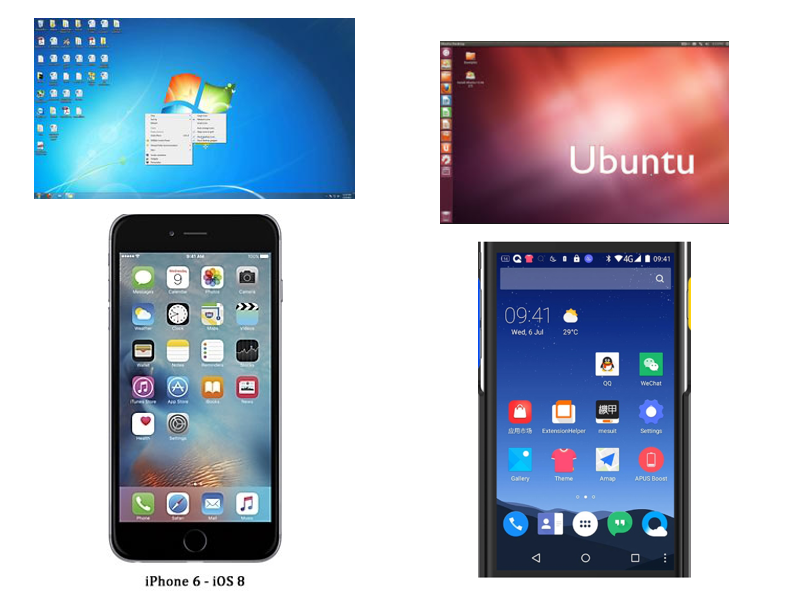
\includegraphics[scale=0.7]{img/C1/1-1/3.png}
		      \caption{常见操作系统}
	      \end{figure}

	\item 程序员:OS是建立在计算机硬件平台上的虚拟机器,它为应用软件提供了许多比计算机硬件功能更强或计算机硬件所没有的功能。

	\item OS开发者:OS是计算机系统中各类资源的管理者,它负责分配、回收以及控制操作系统中的软硬件资源(包括CPU、内存、I/O设备、文件、网络)。

	\item OS开发者:OS是计算机系统工作流程的组织者,它负责协调在系统中运行的各个应用软件的运行次序。
\end{enumerate}

\newpage

\section{OS功能性与非功能性需求}

\subsection{功能性需求}

OS的功能性需求主要有两大类:

\begin{enumerate}
	\item 用户命令:计算机用户需要使用用户命令进行操作,由OS实现的所有用户命令所构成的集合被称为OS的接口(interface)。

	\item 系统调用(system call):应用软件需要使用系统调用来实现OS所提供的服务,由OS实现的所有系统调用所构成的集合被称为应用编程接口(API, Application Programming Interface)。
\end{enumerate}

\subsection{非功能性需求}

OS的非功能性需求主要包括:

\begin{itemize}
	\item 性能 / 效率(performance / efficiency):最大化系统吞吐量(throughput)、最小化响应时间(response time),在分时系统情况下需要满足尽量多的用户。

	\item 公平性(fairness):OS中的算法不能偏向于某些特定类型的进程,但是在某些时候,如实时系统需要及时响应外部事件。

	\item 可靠性(reliability)

	\item 安全性(security)

	\item 可伸缩性(scalability):不同预算可购买不同配置,如个人版和企业版。

	\item 可扩展性(extensibility):OS能够适应新的外部设备的增长。

	\item 可移植性(portability):不能仅限于某一个平台或某一个厂家生产的硬件设备。
\end{itemize}

\newpage

\section{CPU}

\subsection{中央处理器(CPU, Central Process Unit)}

CPU作为计算机系统的运算和控制核心,是信息处理、程序运行的最终执行单元。

\begin{figure}[H]
	\centering
	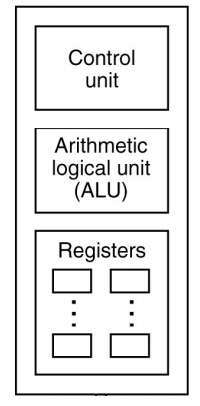
\includegraphics[scale=0.7]{img/C1/1-3/1.png}
	\caption{CPU结构}
\end{figure}

Python中可以通过\lstinline|multiprocessing|模块获取计算机CPU的内核数量。

\begin{lstlisting}[language=Python, title=获取CPU可用数量]
import multiprocessing	# 导入多进程模块
# 获取CPU的可用数量
print("CPU内核数量:%d" % multiprocessing.cpu_count())
\end{lstlisting}

CPU的核心部分有:

\begin{itemize}
	\item  控制单元(CU, Control Unit):控制单元是CPU的子部件,它管理着计算机中所有在这一区域执行的操作。它负责从计算机、指令和数据中获取各种输入,并告诉处理器如何处理它们。

	\item 算术逻辑单元(ALU, Arithmetic and Logic Unit):实现多组算术运算和逻辑运算的组合逻辑电路。

	\item 寄存器(register):寄存器是有限存贮容量的高速存贮部件,它们可用来暂存指令、数据和地址。
\end{itemize}

大多数现代处理器的工作原理是“取指令-译码-执行”(Fetch-Decode-Execute Cycle),也被称为冯·诺依曼架构(Von Neumann Architecture)。

\begin{figure}[H]
	\centering
	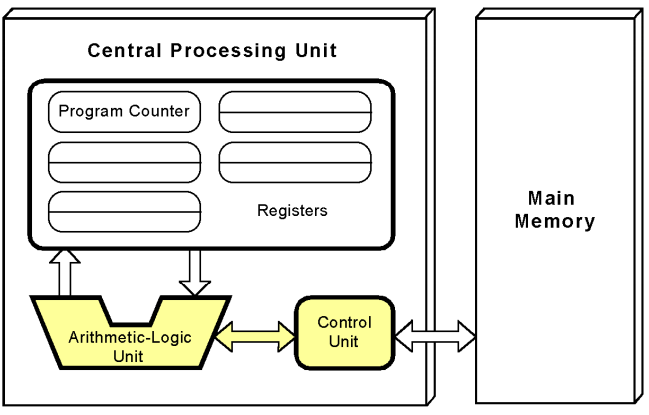
\includegraphics[scale=0.55]{img/C1/1-3/2.png}
	\caption{控制单元CU}
\end{figure}

\begin{figure}[H]
	\centering
	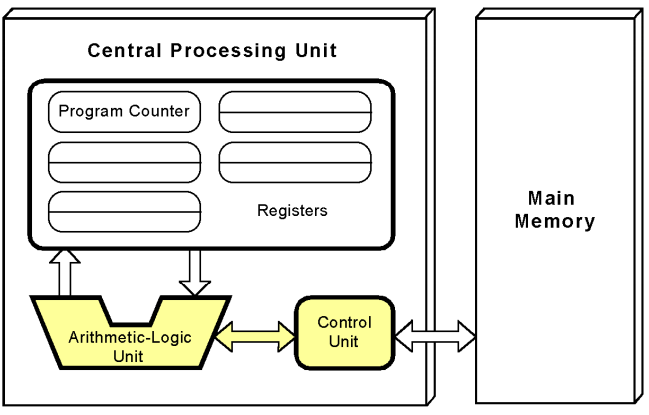
\includegraphics[scale=0.55]{img/C1/1-3/3.png}
	\caption{算术逻辑单元ALU}
\end{figure}

\begin{figure}[H]
	\centering
	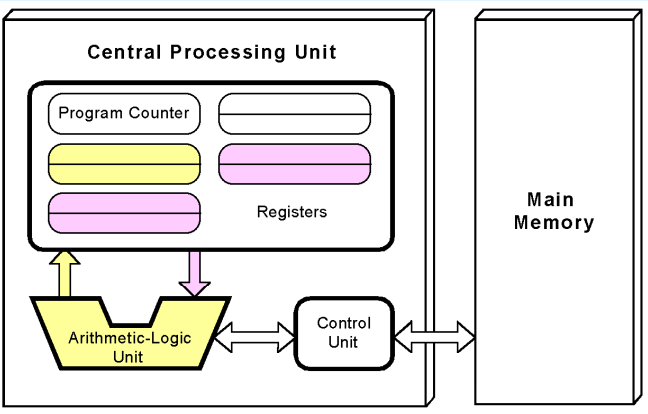
\includegraphics[scale=0.55]{img/C1/1-3/4.png}
	\caption{寄存器register}
\end{figure}

Python中\lstinline|psutil|模块也提供了系统硬件的内容获取。

\begin{lstlisting}[language=Python, title=获取系统硬件信息]
import psutil

def main():
	# CPU信息
	print("【CPU】物理数量:%d"
		% psutil.cpu_count(logical=False))
	print("【CPU】逻辑数量:%d"
		% psutil.cpu_count(logical=True))
	print("【CPU】用户用时:%f"
		% psutil.cpu_times().user)
	print("【CPU】系统用时:%f"、
		% psutil.cpu_times().system)
	print("【CPU】空闲时间:%f"
		% psutil.cpu_times().idle)

if __name__ == "__main__":
	main()
\end{lstlisting}

\newpage

\section{中断}

\subsection{中断(Interrupt)}

中断是指计算机运行过程中,出现某些意外情况需主机干预时,机器能自动停止正在运行的程序并转入处理新情况的程序,处理完毕后又返回原被暂停的程序继续运行。 \\

中断包括鼠标移动、鼠标点击、键盘按键、打印机打印等。 \\

现代计算机中采用中断系统的主要目的是:

\begin{itemize}
	\item 提高计算机系统效率:计算机系统中处理机的工作速度远高于外围设备的工作速度,通过中断可以协调它们之间的工作。当外围设备需要与处理机交换信息时,由外围设备向处理机发出中断请求,处理机及时响应并作相应处理。

	\item 维持系统可靠正常工作:程序员不能直接干预和操纵机器,必须通过中断系统向操作系统发出请求,由操作系统来实现人为干预。在程序运行过程中,如出现越界访问,有可能引起程序混乱或相互破坏信息。为避免这类事件的发生,由存储管理部件进行监测,一旦发生越界访问,向处理机发出中断请求,处理机立即采取保护措施。

	\item 满足实时处理要求:在实时系统中,各种监测和控制装置随机地向处理机发出中断请求,处理机随时响应并进行处理。

	\item 提供故障现场处理手段:处理机中设有各种故障检测和错误诊断的部件,一旦发现故障或错误,立即发出中断请求,进行故障现场记录和隔离,为进一步处理提供必要的依据。
\end{itemize}

\newpage

\section{存储器}

\subsection{存储单位}

计算机存储单位一般使用bit (b)、B、KB、MB、GB、TB、PB、EB、ZB、YB、BB、NB、DB等符号来表示。 \\

位(bit)是计算机最小的存储单位,只存放一位二进制数。 \\

一个字节(byte)为8位二进制数,保存一个英文字母需要一个字节,但保存一个中文需要两个字节字(word)。

\begin{table}[H]
	\centering
	\setlength{\tabcolsep}{5mm}{
		\begin{tabular}{|c|c|}
			\hline
			8 bits     & 1 byte           \\
			\hline
			1024 bytes & 1 Kilobyte (KB)  \\
			\hline
			1024 KB    & 1 Megabyte (MB)  \\
			\hline
			1024 MB    & 1 Gigabyte (GB)  \\
			\hline
			1024 GB    & 1 Terabyte (TB)  \\
			\hline
			1024 TB    & 1 Petabyte (PB)  \\
			\hline
			1024 PB    & 1 Exabyte (EB)   \\
			\hline
			1024 EB    & 1 Zettabyte (ZB) \\
			\hline
			1024 ZB    & 1 Yottabyte (YB) \\
			\hline
		\end{tabular}
	}
	\caption{内存单位转换}
\end{table}

有些硬盘厂商以1000进制为单位,这并不是故意弄虚作假,而是为了设计和制造的方便,直接以1000计算更方便。

\subsection{存储设备}

存储设备是用于储存信息的设备,通常是将信息数字化后再以利用电、磁或光学等方式的媒体加以存储。

\begin{figure}[H]
	\centering
	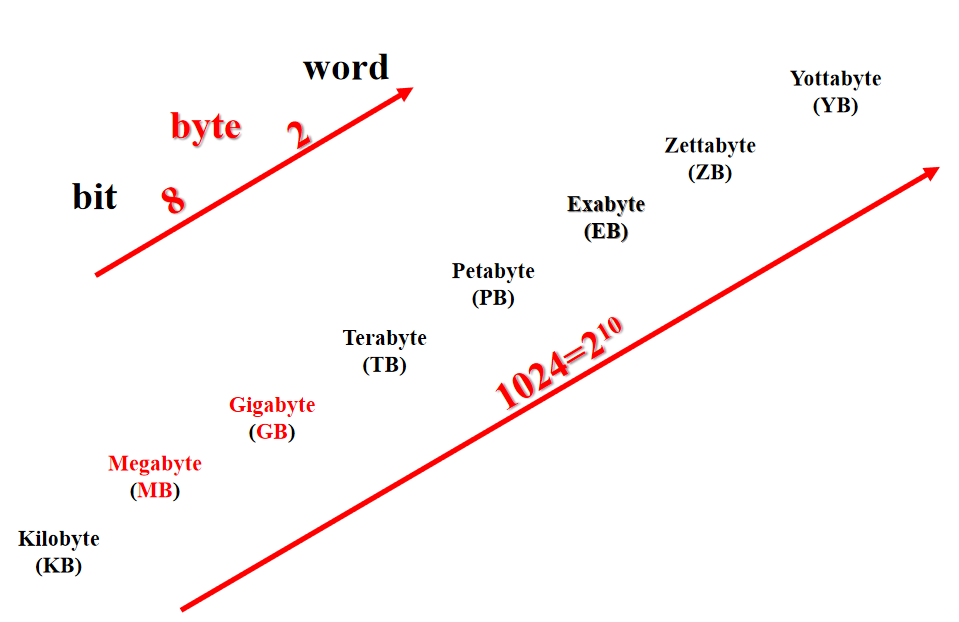
\includegraphics[scale=0.7]{img/C1/1-5/1.png}
	\caption{存储设备}
\end{figure}

\begin{figure}[H]
	\centering
	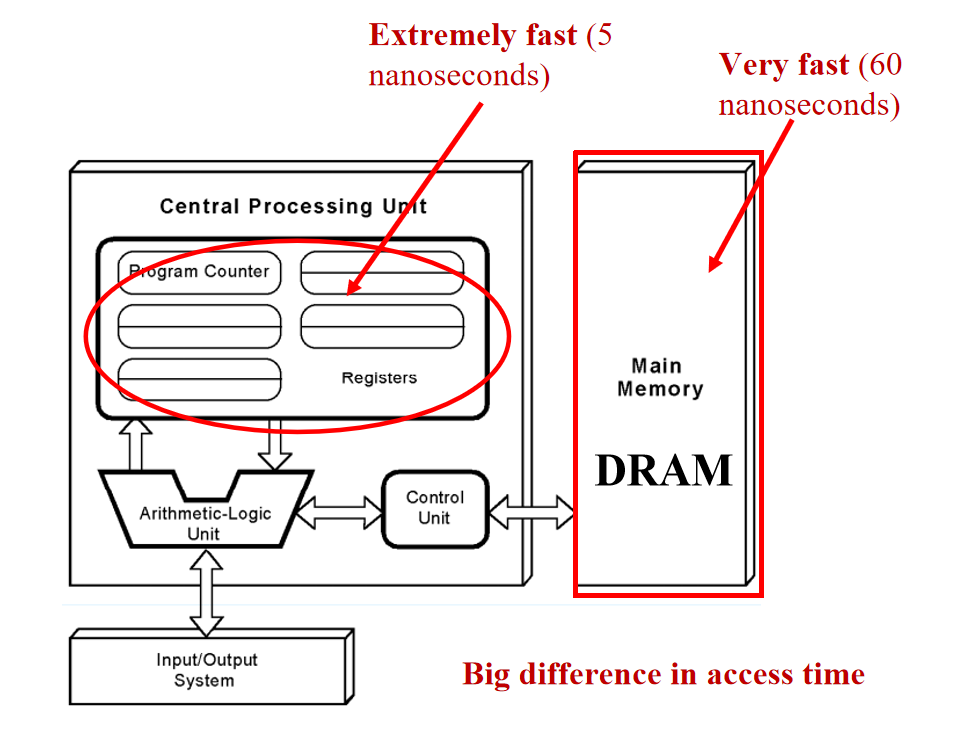
\includegraphics[scale=0.7]{img/C1/1-5/2.png}
	\caption{不同存储设备访问速度对比}
\end{figure}

\subsection{内存缓存(Memory Cache)}

CPU缓存是位于CPU与内存之间的临时存储器,它的容量比内存小的多但是交换速率却比内存要快得多。缓存的出现主要是为了解决CPU运算速率与内存读写速率不匹配的矛盾,因为CPU运算速率要比内存读写速率快很多,这样会使CPU花费很长时间等待数据到来或把数据写入内存。在缓存中的数据是内存中的一小部分,但这一小部分是短时间内CPU即将访问的,当CPU调用大量数据时,就可避开内存直接从缓存中调用,从而加快读取速率。

\begin{figure}[H]
	\centering
	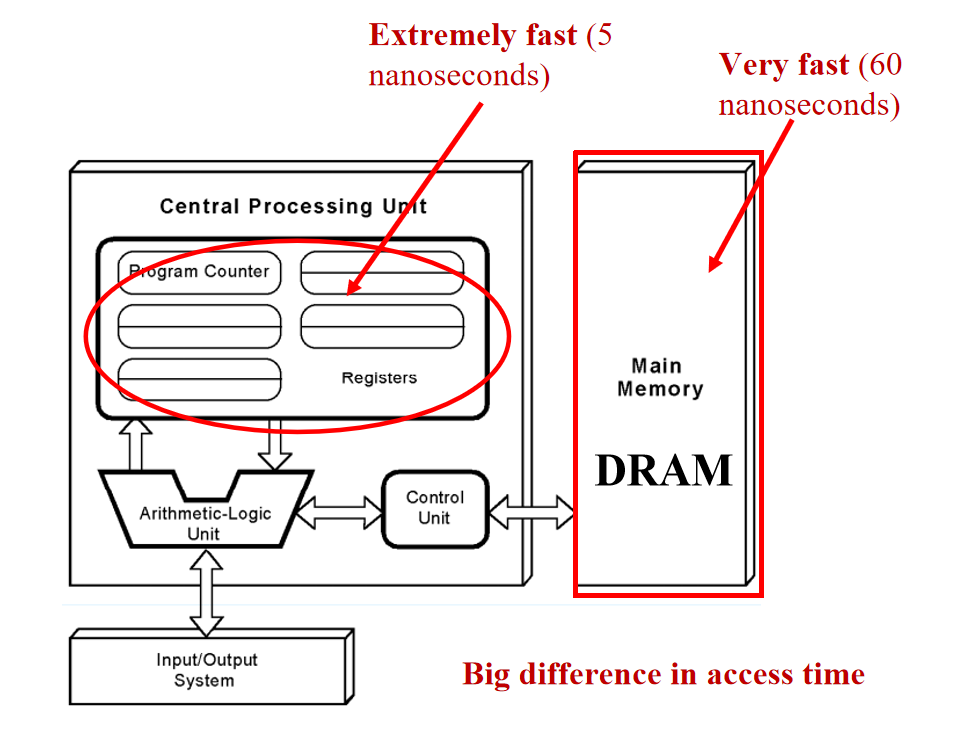
\includegraphics[scale=0.7]{img/C1/1-5/3.png}
	\caption{内存缓存}
\end{figure}

\newpage

\section{操作系统演变}

\subsection{串行处理(Serial Processing)}

操作系统一直在不断地更新版本,版本升级就是操作系统的改变。操作系统改变的原因包括修复漏洞、支持新的服务、硬件升级、提升性能等。 \\

串行处理时期的计算机体积非常大,因为没有操作系统,所以操作的时候需要通过扳动按钮,最终通过灯来进行显示。这种计算机必须全部由专家操作,一般用户是用不了这台计算机的。

\begin{figure}[H]
	\centering
	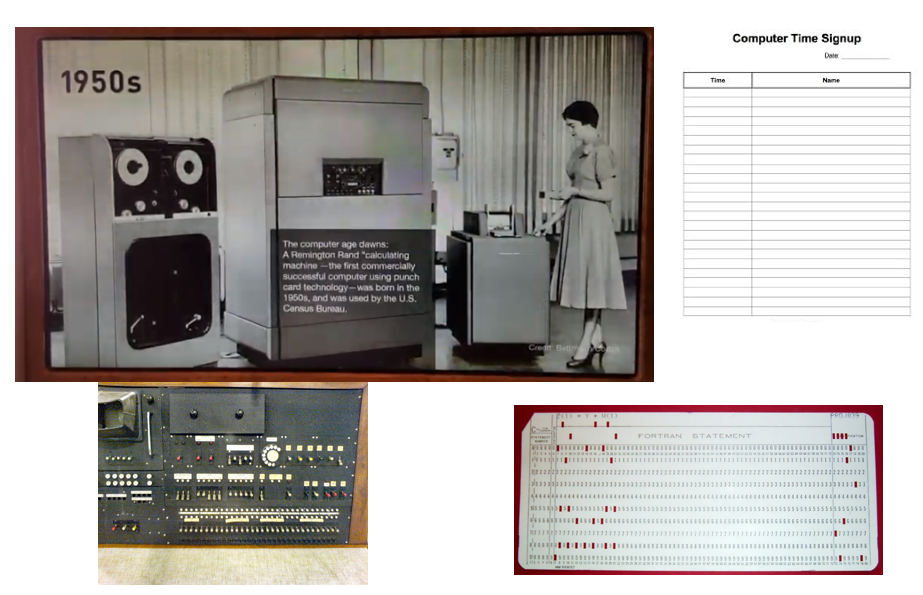
\includegraphics[scale=0.7]{img/C1/1-6/1.png}
	\caption{串行处理}
\end{figure}

这就导致了两个主要的问题:

\begin{enumerate}
	\item 调度低效:机器需要等待人扳动按钮,浪费时间。
	\item 启动时间慢:没有自动化,需要手工装入编译器、源程序、保存中间代码等。
\end{enumerate}

\subsection{单道批处理系统(Simple Batch System)}

单道批处理系统可以说是第一代操作系统,在外存中可以有一批作业等待,当内存没有作业可运行的时候,Monitor就会从外存去选一个作业进入内存。最简单选择方式就是按队列顺序选择,但这不一定是最合理的,这就涉及到了调度算法。

\subsection{多道程序系统(Multiprogramming)}

一个支持Multiprogramming的系统允许多道程序同时准备运行。当正在运行的那道程序因为某种原因(比如等待输入或输出数据)暂时不能继续运行时,系统将自动地启动另一道程序运行。一旦原因消除(比如数据已经到达或数据已经输出完毕),暂时停止运行的那道程序在将来某个时候还可以被系统重新启动继续运行。

\begin{figure}[H]
	\centering
	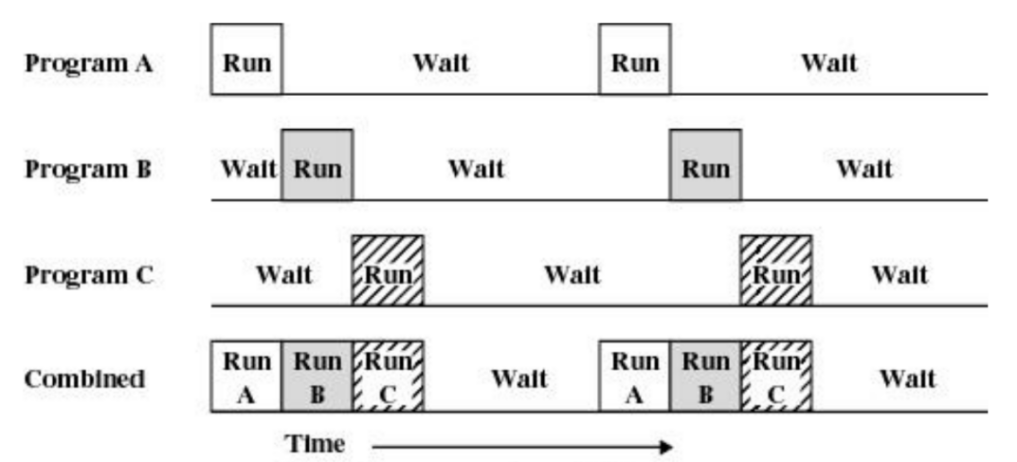
\includegraphics[]{img/C1/1-6/2.png}
	\caption{多道程序系统}
\end{figure}

\subsection{并发编程(Concurrent)}

并发编程是一种有效提高操作系统(服务器)性能的技术手段,现代的操作系统之中最为重要的代表就是并发性,例如现在的CPU都属于多核CPU。 \\

早期的DOS操作系统有一个非常重要的特征:一旦系统沾染了病毒,那么所有的程序就无法直接执行了。因为传统的DOS系统属于单进程模型,在同一个时间段上只能运行一个程序,病毒程序运行了,其它程序自然就无法运行。 \\

后来到了Windows操作系统,即便有病毒,也可以正常执行。这采用的是多进程的编程模型,同一时间段上可以同时运行多个程序。

\begin{figure}[H]
	\centering
	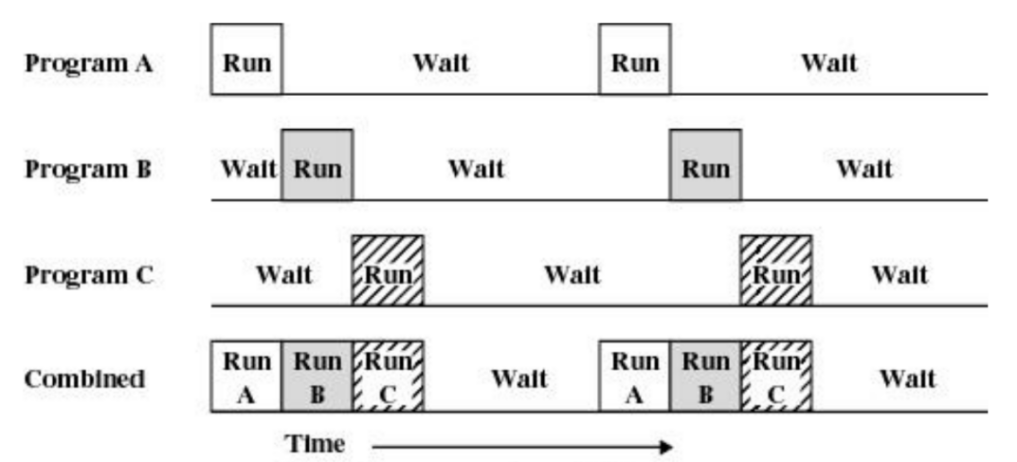
\includegraphics[scale=0.6]{img/C1/1-6/3.png}
	\caption{并发编程}
\end{figure}

只要打开Windows的任务管理器,就可以直接清楚发现所有正在执行的并行进程。

\begin{figure}[H]
	\centering
	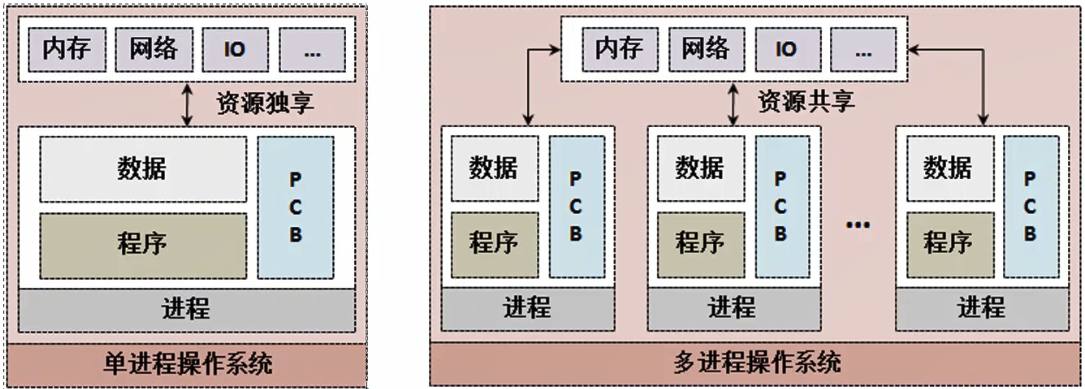
\includegraphics[scale=0.7]{img/C1/1-6/4.png}
	\caption{任务管理器}
\end{figure}

在早期的硬件系统之中由于没有多核CPU的设计,利用时间片的轮转算法(Round Robin),保证在同一个时间段可以同时执行多个进行,但是在某一个时间点上只允许执行一个进程,可以实现资源的切换。

\begin{figure}[H]
	\centering
	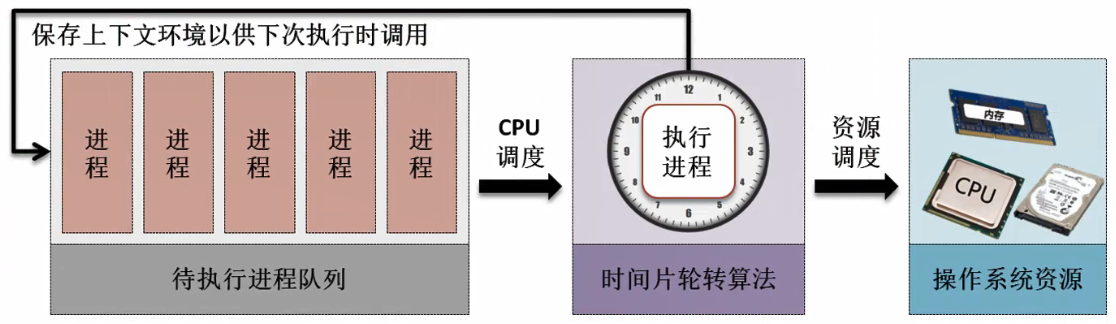
\includegraphics[scale=0.6]{img/C1/1-6/5.png}
	\caption{时间片轮转算法}
\end{figure}

服务器的硬件性能是有限的,但是对于大部分的程序来讲都属于过剩的状态。于是如果按照传统的单进程模式来运行程序,所有的硬件资源几乎都会被浪费。

\subsection{分时系统(Time-Sharing System)}

分时系统首先是个多道系统,分时在多道的基础上对每个任务以时间为固定切片,时间到了就切换到下一个任务。这种系统非常适合于交互式系统,例如访问网络服务器,采用时间片轮转的方式同时为几十个、几百个用户服务。

\begin{figure}[H]
	\centering
	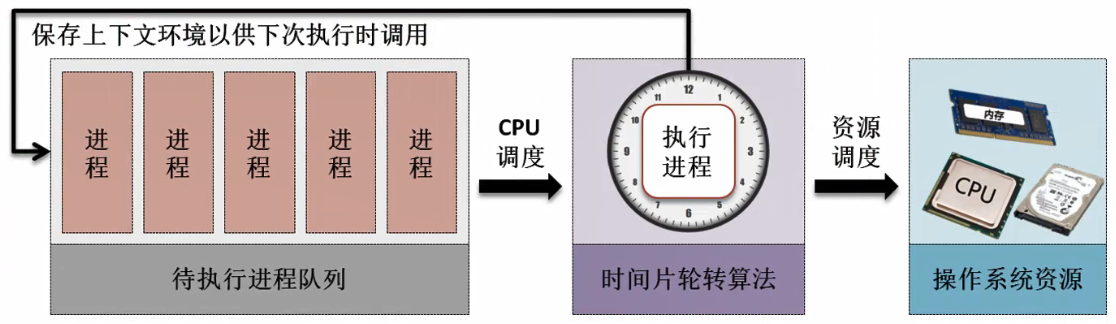
\includegraphics[scale=0.55]{img/C1/1-6/6.png}
	\caption{分时系统}
\end{figure}

分时系统会有一些问题,比如时间片太短会频繁的中断,造成很大的系统开销,或者有些任务不能被中断,被中断后可能恢复不了。所以分时系统是在某些需求的环境下才会提供。

\subsection{移动系统(Mobile System)}

移动设备体积小,可以手持便于携带。移动设备一般都具有LED平板界面,提供数字化按钮和键盘的触摸屏界面。移动设备操作系统的例子包括Apple iOS、Google Android、Research in Motion's BlackBerry OS等。

\newpage